\documentclass[12pt, pdf, hyperref={unicode},handout]{beamer}

\mode<presentation>
{
  \usetheme{Madrid}       % or try default, Darmstadt, Warsaw, ... Madrid
  \usecolortheme{default} % or try albatross, beaver, crane, ...default
  \usefonttheme{serif}    % or try default, structurebold, ... serif
  \usefonttheme{professionalfonts}
  \setbeamertemplate{navigation symbols}{}
% \setbeamertemplate{caption}[numbered]
} 

\usepackage[english,russian]{babel}
\usepackage[utf8x]{inputenc}
\usepackage{hyperref}
\graphicspath{{image/}}
\definecolor{links}{HTML}{2A1B81}
\hypersetup{colorlinks,linkcolor=,urlcolor=links}
\usepackage{listings}
\usepackage{concmath}
\usepackage{ragged2e}
\renewcommand{\raggedright}{\leftskip=0pt \rightskip=0pt plus 0cm}
\usepackage[orientation=landscape,size=A4, scale=4]{beamerposter}
\usepackage{enumerate}
\usepackage[T2A]{fontenc}
\usepackage{subfigure}
\usepackage{float}
\usepackage{setspace}
\usepackage{array,longtable}

\usepackage{comment}

\lstset{
language=python,
basicstyle=\small\sffamily, % размер и начертание шрифта для подсветки кода
%numbers=left,               % где поставить нумерацию строк (слева\справа)
%numberstyle=\tiny,           % размер шрифта для номеров строк
stepnumber=1,                   % размер шага между двумя номерами строк
%numbersep=5pt,                % как далеко отстоят номера строк от подсвечиваемого кода
backgroundcolor=\color{white}, % цвет фона подсветки - используем \usepackage{color}
showspaces=false,            % показывать или нет пробелы специальными отступами
showstringspaces=false,      % показывать или нет пробелы в строках
showtabs=false,             % показывать или нет табуляцию в строках
frame=single,              % рисовать рамку вокруг кода
tabsize=2,                 % размер табуляции по умолчанию равен 2 пробелам
captionpos=t,              % позиция заголовка вверху [t] или внизу [b] 
breaklines=true,           % автоматически переносить строки (да\нет)
breakatwhitespace=false, % переносить строки только если есть пробел 
extendedchars=true,
inputencoding=utf8x,
commentstyle=\itshape,
stringstyle=\bf,
extendedchars=false,
keepspaces = true,
belowcaptionskip=5pt }


\newtheorem{hyp}{Гипотеза}
\newtheorem{theor}{Теорема}
\newtheorem{dfn}{Определение}
\newtheorem{resume}{Следствие}
\newtheorem{exmpl}{Пример}


% Here's where the presentation starts, with the info for the title slide
\title[Лекция 2]{\Huge{Автоматные грамматики и конечные автоматы}}
\author[\textcopyright   Артамонов Ю.Н.]{}
\institute[]{}
\date{}

\begin{document}

\begin{frame}
  \titlepage
\end{frame}

% These three lines create an automatically generated table of contents.
\begin{frame}{Содержание}
  \tableofcontents
\end{frame}

\section{Автоматные грамматики}


\begin{frame}{Понятие регулярной грамматики}
  \begin{block}

    \small{
      Как известно из прошлой лекции, наиболее простой тип грамматик - \textit{автоматные грамматики}. Их правила определяются продукциями вида $A\rightarrow a|aB|\epsilon$.  Здесь $A, B$ - это один какой-либо нетерминальный символ из нетерминального алфавита, $a$ - один какой-либо терминальный символ из терминального алфавита.

      В более общем случае говорят о \textit{регулярных грамматиках}, в которых символ $a$ может состоять не из одного терминального символа, а быть цепочкой терминальных символов (обозначим его $\gamma\in \Sigma^*$). В свою очередь выделяют два класса регулярных грамматик: \textit{праволинейная регулярная грамматика} (в правиле $A\rightarrow \gamma B$ нетерминальный символ $B$ стоит справа);  \textit{леволинейную регулярную грамматику}, если в правиле $A\rightarrow B \gamma$ нетерминальный символ $B$ стоит слева.

      Доказано, что эти два класса грамматик эквивалентны: для любого регулярного языка, заданного праволинейной грамматикой, можно построить леволинейную грамматику, задающую тот же язык, и наоборот.

      Разница между леволинейными и праволинейными грамматиками заключается в основном в том, в каком порядке строятся предложения языка: слева направо для леволинейных и справа налево для праволинейных.


}

  \end{block}
  
\end{frame}

\begin{frame}{Понятие регулярной грамматики}
  \begin{block}

    \small{
      Рассмотрим простой пример: $S\rightarrow\epsilon|aaS|abT, T\rightarrow abT|bbS$. Данная грамматика, как видно праволинейная регулярная грамматика. Посмотрим, возможен ли в этой грамматике вывод цепочки $aaababbb$. Чтобы восстановить этот вывод, мы должны двигаться справа налево:
      $$aaababbb\rightarrow aaababbb\epsilon\rightarrow aaababbbS\rightarrow aaababT\rightarrow aaabT\rightarrow aaS\rightarrow S$$
      Данная цепочка вывода - это основная задача так называемого лексического анализатора. Как мы видим, он вынужден двигаться в своем выводе справа налево (каждый раз он заменяет на нетерминальный символ цепочку терминальных символов справа).
      Это не всегда удобно, так как лексическому анализатору нужно анализировать цепочку с конца входной строки. Поэтому обычно используют леволинейные регулярные грамматики.

      В тоже время еще более простая жизнь для лексического анализатора наступает в случае автоматных грамматик, которые, как следует из определений, являются частным случаем регулярных грамматик. В чистых автоматных грамматиках обычно еще убирают правило $A\rightarrow \epsilon$ и оставляют только правила $A\rightarrow a|aA$. Аналогично, автоматные грамматики могут быть право и леволинейными.

}

  \end{block}
  
\end{frame}

\begin{frame}{Преобразование регулярной грамматики к автоматному виду}
  \begin{block}

    \small{
      Оказывается, класс автоматных грамматик почти эквивалентен регулярным грамматикам. Для полной эквивалентности необходимо в автоматную грамматику добавить еще одно правило $S\rightarrow \epsilon$, где $S$ - целевой символ, при этом символ $S$ не должен встречаться в правых частях других правил. На практике реально используемые языки не содержат, как правило, пустую цепочку, поэтому автоматные и регулярные грамматики обычно отождествляют.

      Существует алгоритм преобразования регулярной грамматики к автоматному виду. Рассмотрим данный алгоритм на примере введеной праволинейной регулярной грамматики: $S\rightarrow\epsilon|aaS|abT, T\rightarrow abT|bbS$. Очевидно, что каждое правило $S\rightarrow aaS, S\rightarrow abT, T\rightarrow abT, T\rightarrow bbS$ нужно представить цепочкой правил:
      $$S\rightarrow aaS\Rightarrow S\rightarrow aS_1, S_1\rightarrow aS$$
      Аналогично поступаем в остальных случаях:   $$S\rightarrow abT\Rightarrow S\rightarrow aT_1, T_1\rightarrow bT$$
      $$T\rightarrow abT\Rightarrow T\rightarrow aT_2, T_2\rightarrow bT$$
      $$T\rightarrow bbS\Rightarrow T\rightarrow bT_3, T_3\rightarrow bS$$
Чтобы устранить правило $S\rightarrow \epsilon$, нужно реализовать возможность получить $S\rightarrow aa$ и $T\rightarrow bb$, что также легко сделать: $S\rightarrow aS_2, S_2\rightarrow a, T\rightarrow bT_4, T_4\rightarrow b$
}

  \end{block}
  
\end{frame}

\begin{frame}{Преобразование регулярной грамматики к автоматному виду}
  \begin{block}

    \small{
      Окончательно, грамматика с набором правил: $S\rightarrow aS_1, S_1\rightarrow aS, S\rightarrow aT_1, T_1\rightarrow bT, T\rightarrow aT_2, T_2\rightarrow bT, T\rightarrow bT_3, T_3\rightarrow bS, S\rightarrow aS_2, S_2\rightarrow a, T\rightarrow bT_4, T_4\rightarrow b$ является праволинейной автоматной грамматикой, которая порождает тот же язык, что и регулярная грамматика $S\rightarrow\epsilon|aaS|abT, T\rightarrow abT|bbS$.

      С автоматными грамматиками жить становится действительно легче, поскольку порождаемые ими цепочки можно распознавать специальными устройствами-распознавателями, которые получили название \textbf{конечные автоматы}. 

}

  \end{block}
  
\end{frame}

\section{Конечные автоматы}

\begin{frame}{Неформальное определение конечного автомата}
  \begin{block}

    \small{
      Конечные автоматы являются моделью для многих компонентов аппаратного и программного обеспечения. Ниже представлены наиболее важные примеры их использования:
      \begin{enumerate}
\item{Программное обеспечение, используемое для разработки и проверки цифровых
схем.}
\item{Лексический анализатор стандартного компилятора, т.е. тот компонент компилятора, который отвечает за разбивку исходного текста на такие логические единицы, как идентификаторы, ключевые слова и знаки пунктуации.}
\item{Программное обеспечение для сканирования таких больших текстовых массивов, как наборы Web-страниц, с целью поиска заданных слов, фраз или других последовательностей символов (шаблонов).}
\item{Программное обеспечение для проверки различного рода систем (протоколы связи или протоколы для защищенного обмена информацией), которые могут находиться в конечном числе различных состояний.}
\end{enumerate}
В целом конечный автомат можно определить как устройство, которое под воздействием входного алфавита переходит в какое-либо состояние из некоторого конечного множества, учитывая, в каком состоянии это устройство находится в текущим момент времени.
}

  \end{block}
  
\end{frame}

\begin{frame}{Примеры конечных автоматов}
  \begin{block}

    \small{
      Примером простейшего конечного автомата может быть кнопка включения, выключения - в зависимости от того, в каком состоянии кнопка, повторное нажатие может привести к включению или выключению света. Конечные автоматы удобно иллюстрировать в виде диаграммы переходов из состояния в состояние. Например, вот так можно представить автомат - <<Кнопка>>.
      \begin{figure}[htb] 
    \centering
    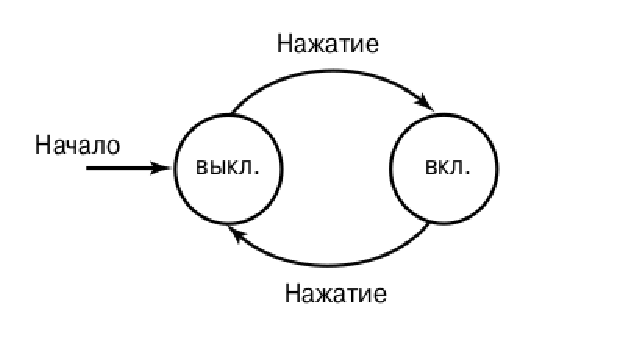
\includegraphics [scale=1.0]{ris1.eps}
  \end{figure}

  Более интересным примером является автомат по продаже газировки. Предположим, он работает по следующим правилам:
  \begin{itemize}
  \item{Автомат распознает монеты достоинством 1, 2, 3 доллара.}
  \item{Если автомат получил в сумме 3 доллара, он продает газировку.}
  \item{Если автомат получил меньше 3 долларов, он ожидает.}
    \item{Если автомат получил больше 3 долларов, он возвращает деньги.}
    
    \end{itemize}
}

  \end{block}
  
\end{frame}

\begin{frame}{Примеры конечных автоматов}
  \begin{block}

    \small{
      Ниже на рисунке показана диаграмма работы автомата по продаже газировки.
      \begin{figure}[htb] 
    \centering
    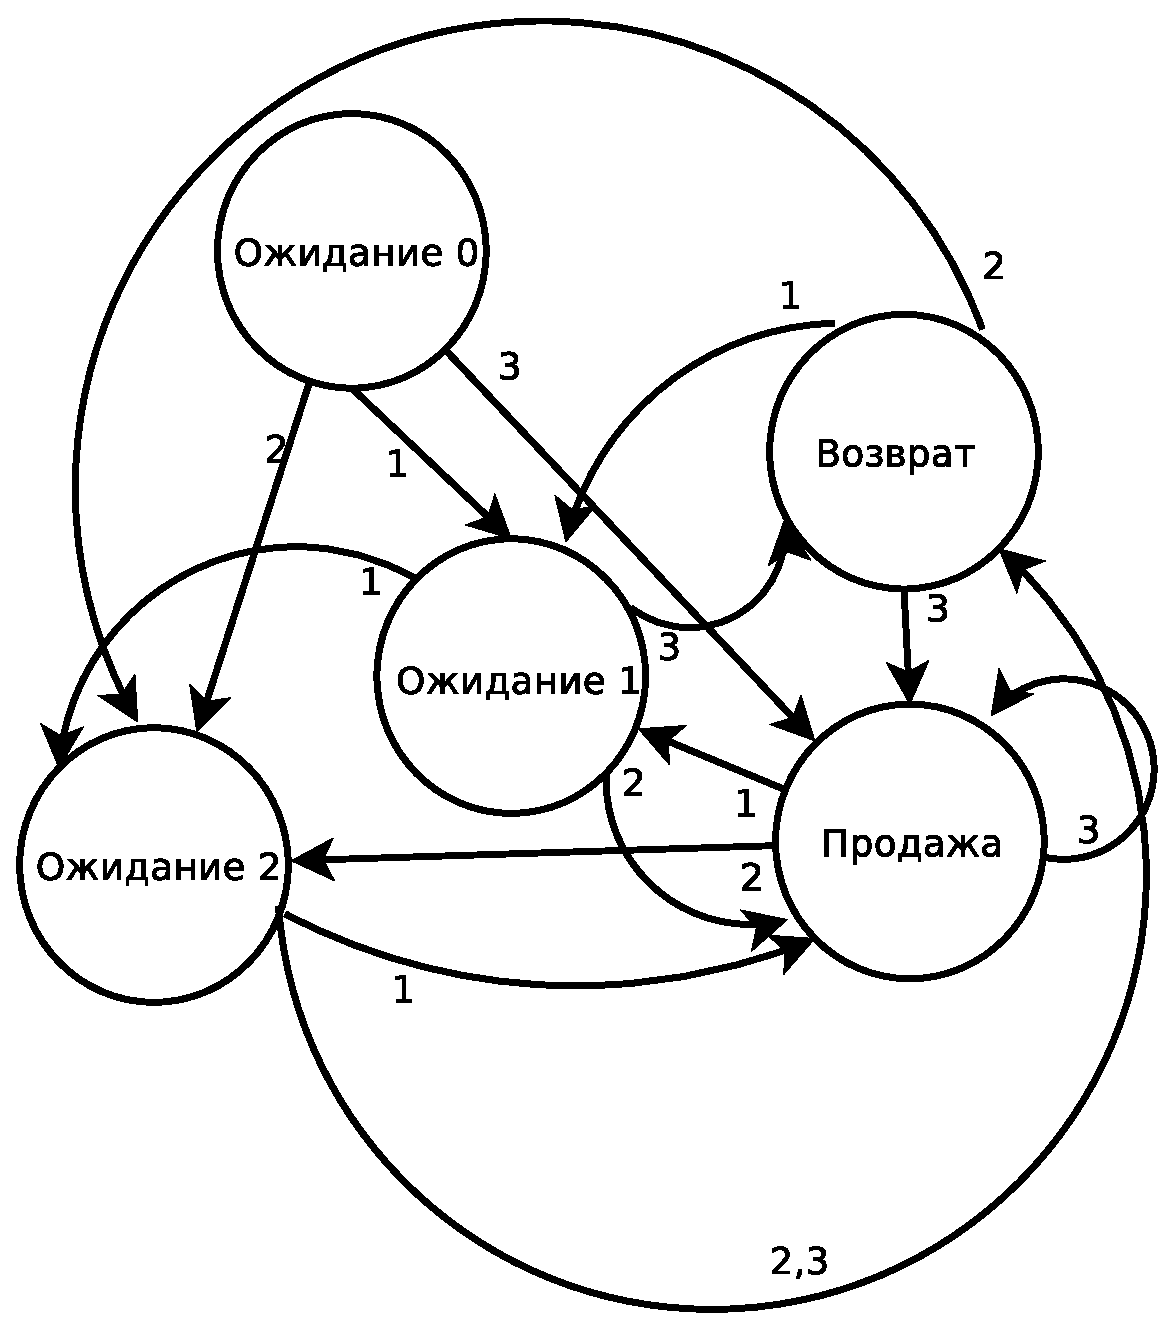
\includegraphics [scale=0.7]{ris2.eps}
  \end{figure}
}

  \end{block}
  
\end{frame}

\begin{frame}{Пример синтеза порождающей грамматики для конечного автомата}
  \begin{block}

    \small{
      Можно попробовать построить порождающую грамматику языка, который распознает данный автомат. Для этого примем соглашение, что наш автомат распознает входную цепочку из терминальных символов алфавита $\{1, 2, 3\}$, если по окончанию этой цепочки автомат будет находиться в состоянии <<Продажа>>. Например, цепочки $111, 1222111, 333$ распознаются, а цепочки $1112, 1322, 222$ не распознаются.

      Обозначим  состояние <<Продажа>> нетерминалом $S$. Будем считать, что если ничего не подается, автомат успешно это распознает. Состояние <<Ожидание 1>> обозначим нетерминальным символом $A$, состояние <<Ожидание 2>> обозначим нетерминальным символом $B$, состояние <<Возврат>> обозначим нетерминальным символом <<C>>. Ясно, что из начального состояния $S$ под действием терминальных символов $1,2,3$ автомат переходит в состояния $A,B,S$ соответственно. Это дает следующие продукции $$S\rightarrow 1A|2B|3S|\epsilon$$
      
}

  \end{block}
  
\end{frame}

\begin{frame}{Пример синтеза порождающей грамматики для конечного автомата}
  \begin{block}

    \small{
      
      Из состояния $A$ под действием $1,2,3$ автомат переходит  в состояния $B,S,C$ соответственно: $$A\rightarrow 1B|2S|3C$$
      Из состояния $B$ под действием $1,2,3$ автомат переходит  в состояния $S,C,C$ соответственно: $$B\rightarrow 1S|2C|3C$$
      Наконец, из состояния $C$ под действием $1,2,3$ автомат переходит  в состояния $A,B,S$ соответственно:$$C\rightarrow 1A|2B|3S$$
      Окончательно, порождающая грамматика состоит из следующих продукций:
      $$S\rightarrow 1A|2B|3S|\epsilon, A\rightarrow 1B|2S|3C, B\rightarrow 1S|2C|3C, C\rightarrow 1A|2B|3S$$
Мы построили порождающую грамматику на основе неких интуитивных представлений о том, как работает наш автомат. Однако, эти интуитивные представления не всегда доступны. Для надежности нужен более формальный подход. Для этого введем более строгое определение конечного автомата.
}

  \end{block}
  
\end{frame}

\begin{frame}{Формальное определение конечного автомата}
  \begin{block}

    \small{
      \begin{dfn}
        \textbf{Конечным автоматом} называют кортеж из пяти элементов:
        $$A=<Q, \Sigma, \delta, q_0, F>$$
        $Q$ - конечное множество состояний автомата.

        $\Sigma$ - конечное множество входных символов (алфавит автомата).

        $\delta$ - функция перехода из одного состояния в другое состояние под действием символа из $\Sigma$.

        $q_0$ - начальное состояние автомата, в котором он находится перед началом работы $q_0\in Q$.

        $F$ - непустое множество конечных состояний автомата, в которых он должен находиться по окончанию работы $F\subseteq Q, F\neq \emptyset$
        \end{dfn}
     Автомат является полностью определенным, если в каждом его состоянии существует функция перехода для всех возможных входных символов. 
}

  \end{block}
  
\end{frame}

\begin{frame}{Формальное определение конечного автомата}
  \begin{block}

    \small{
      Работа конечного автомата представляет собой последовательность шагов. На каждом таким шаге автомат находится в одном из своих состояний, на следующем шаге он переходит в следующее состояние (может остаться в этом же состоянии) под действием входного символа. Такой переход задается функцией переходов $\delta$. Работа автомата продолжается до тех пор, пока на его вход поступают символы. Если по окончанию входных символов автомат находится в одном из конечных состояний множества $F$, то говорят, что автомат распознал входную цепочку символов - она допустима в том языке, который понимает конечный автомат, в противном случае такая цепочка не распознается и считается недопустимой цепочкой этого языка.

      Рассмотрим пример автомата по продаже газировки. Обозначим для краткости <<Ожидание 0>> состоянием $A$,  <<Ожидание 1>> состоянием $B$, <<Ожидание 2>> состоянием $C$, <<Возврат>> состоянием $D$, <<Продажа>> состоянием $F$. Имеем:
      $$\delta(A,1)=B, \delta(A,2)=C, \delta(A,3)=F, \delta(B,1)=C, \delta(B,2)=F, \delta(B,3)=D$$
      $$\delta(C,1)=F, \delta(C,2)=D, \delta(C,3)=D, \delta(D,1)=A, \delta(D,2)=B, \delta(D,3)=F$$
      $$\delta(F,1)=A, \delta(F,2)=B, \delta(F,3)=F$$
      Как видно, автомат полностью определен,при этом $q_0=A$, а состоние $F$ является единственным конечным состоянием, $\Sigma=\{1,2,3\}$.
}

  \end{block}
  
\end{frame}

\begin{frame}{Формальное определение конечного автомата}
  \begin{block}

    \small{
      Конечный автомат часто представляют в виде диаграммы или графа переходов по аналогии с тем, как мы рисовали автоматы. Граф переходов конечного автомата - это направленный граф, в котором вершины помечены символами состояний автомата, а дуги помечены символами входного алфавита. Начальное состояние помечается дополнительной пунктирной линией, конечное состояние - дополнительной сплошной линией. На рисунке представлен пример.
       \begin{figure}[htb] 
    \centering
    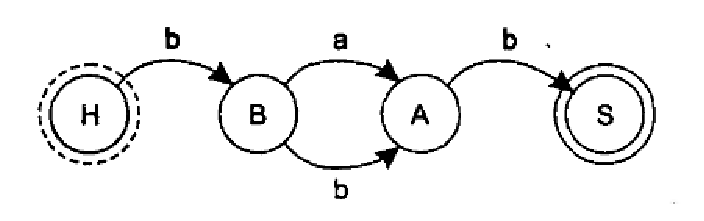
\includegraphics [scale=0.7]{ris3.eps}
  \end{figure}

  Ясно, что этой диаграмме соответствует конечный автомат $A=<\{H, A, B, S\}, \{a,b\}, \delta, H, \{S\}>, \delta: \delta(H,b)=B, \delta(B,a)=A, \delta(B,b)=A, \delta(A,b)=S$

  Однако, как видно данный автомат не является полностью определен. На практике для полной определенности добавляют еще одно состояние, которое можно назвать <<Ошибка>>. На это состояние замыкают все неопределенные переходы. Пример такой модификации представлен ниже:
       \begin{figure}[htb] 
    \centering
    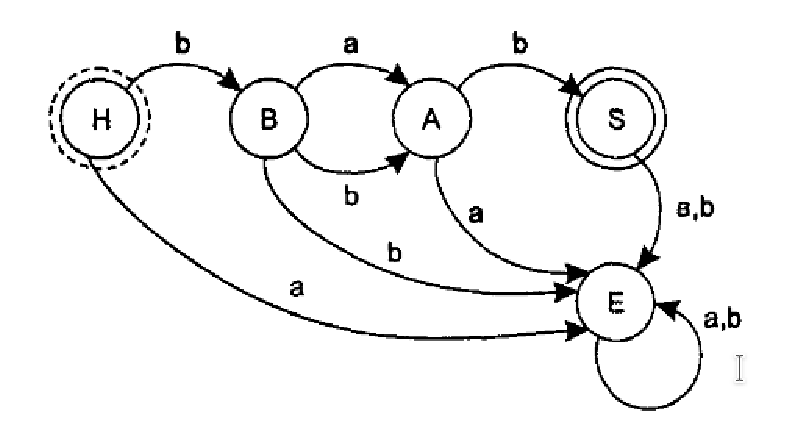
\includegraphics [scale=0.5]{ris4.eps}
  \end{figure}
}

  \end{block}
  
\end{frame}

\begin{frame}{Детерминированные и недетерминированные конечные автоматы}
  \begin{block}

    \small{
      Важной особенностью функции переходов является ее однозначность - когда для одного и того же состояния под действием одного и того же символа автомат переходит в одно единственное состояние. В этом случае автомат называется \textbf{детерминированным}, в противном случае он называется \textbf{недетерминированным}. Для недетерминированных автоматов функция переходов задает множество возможных состояний, в которые может перейти автомат. Например, автомат с функцией переходов $\delta(H,b)=B, \delta(B,a)=A,\delta(A,b)=\{B,S\}$ является недетерминированным из-за перехода вида $\delta(A,b)=\{B,S\}$.

      В принципе на практике часто используют недетерминированные конечные автоматы. Они являются более выразительными, однако для автоматизации операций синтеза анализаторов целесообразно переходить от недетерминированных конечных автоматов к детерминированным. Данный алгоритм мы рассмотрим позже, а сейчас рассмотрим, как по произвольному автомату получить порождающую грамматику.
}

  \end{block}
  
\end{frame}

\begin{frame}{Построение автоматной грамматики по конечному автомату}
  \begin{block}

    \small{
      Задача формулируется таким образом: имеется конечный автомат $A=<Q,\Sigma, \delta, q_o, F>$, необходимо построить эквивалентную ему леволинейную грамматику $G(T,N,S,R)$.
      \begin{enumerate}
      \item{Принимаем $T=\Sigma$.}
      \item{Принимает $T=Q\setminus\{q_0\}$ - множество терминальных символов совпадает с множеством состояний автомата, исключая начальное состояние.}
      \item{Для каждого перехода конечного автомата $\delta(A,t)=\{B_1,B_2,\ldots,B_n\}$ добавляем следующие правила:
          \begin{itemize}
          \item{Если $A=q_o$, то добавляем правила $B_i\rightarrow t, i=1,\ldots, n$}
          \item{Если $A\neq q_o$, то добавляем правила $B_i\rightarrow At, i=1,\ldots, n$}
            \end{itemize}
            \item{Если множество конечных состояний содержит только одно состояние $F=\{F_0\}$, то целевым символом S принимаем $F_0$.  Если $F=\{F_1, F_2,\ldots, F_n\}$, то целевым символом принимаем $S$ и добавляем правило $S\rightarrow F_1,|F_2|\ldots| F_n$.}
            
        }
        
        \end{enumerate}

      }
  \end{block}
  
\end{frame}

\begin{frame}{Построение автоматной грамматики по конечному автомату}
  \begin{block}

    \small{
      Преобразуем в качестве примера автомат по продаже газировки в автоматную грамматику:
      $$\delta(A,1)=B, \delta(A,2)=C, \delta(A,3)=F, \delta(B,1)=C, \delta(B,2)=F, \delta(B,3)=D$$
      $$\delta(C,1)=F, \delta(C,2)=D, \delta(C,3)=D, \delta(D,1)=A, \delta(D,2)=B, \delta(D,3)=F$$
      $$\delta(F,1)=A, \delta(F,2)=B, \delta(F,3)=F$$

      Имеем: $T=\{1,2,3\}, N=\{B,C,D,F\}, S=F$, у автомата состояние $A$ принято за начальное.
      \begin{itemize}
      \item{$B\rightarrow 1, C\rightarrow 2, S\rightarrow 3$}
      \item{$C\rightarrow B1, S\rightarrow B2, D\rightarrow B3$}
      \item{$S\rightarrow C1, D\rightarrow C2|C3$}
      \item{$B\rightarrow B2, S\rightarrow D3$}
        \item{$B\rightarrow S2, S\rightarrow S3$}
        \end{itemize}
        }

  \end{block}
  
\end{frame}

\begin{frame}{Построение конечного автомата по автоматной леволинейной грамматике}
  \begin{block}

    \small{
      Возможен и обратный алгоритм:
      \begin{enumerate}
      \item{$Q=N\cup \{H\}$ - множество состояний совпадает с множеством нетерминалов с добавлением начального состояния.}
      \item{$\Sigma=T$.}
      \item{Если встречается правило $A\rightarrow t$, то в функцию переходов $\delta(H,t)$ добавляем состояние $A$.}
      \item{Если встречается правило $A\rightarrow Bt$, то в функцию переходов $\delta(B,t)$ добавляем состояние $A$.}
      \item{$q_0=H$.}
        \item{$F=\{S\}$.}
        
        \end{enumerate}
        }

  \end{block}
  
\end{frame}

\begin{frame}{Задача}
  \begin{block}

    \small{
      Придумать автоматную грамматику работы лифта (он считается трехэтажным, с первого этажа можно подняться на любой, с любого можно только спуститься на  первый), построить по ней конечный автомат или решить обратную задачу.
        }

  \end{block}
  
\end{frame}


\begin{frame}[fragile]{Пример построения программного синтезатора на основе порождающей грамматики}
 
\begin{lstlisting}[language=python]
import random
class gramm:
    __rules=[]
    def add_rule(self, S):
        self.__rules.append(S)
    def look(self):
        return self.__rules
    def deduct(self, L, n):
        while (n!=0):
            r=random.randint(0, len(self.__rules)-1)
            st=self.__rules[r]
            if L.find(st[0])!=-1:
                print(st)
                L=L.replace(st[0],st[1])
            n-=1
        return L
    \end{lstlisting}

  \end{frame}
 



\end{document}
